\documentclass{beamer}

\mode<presentation>
{
  \usetheme{Frankfurt}
  \usecolortheme{orchid}
  \setbeamercovered{invisible}
  \setbeamertemplate{footline}[frame number]
}

\usepackage[english]{babel}
\usepackage[latin1]{inputenc}
\usepackage{times}
\usepackage[T1]{fontenc}
\usepackage{tikz}
\usepackage{array}
\usepackage{cancel}


\usetikzlibrary{shapes,backgrounds}

\def\multiset#1#2{\ensuremath{\left(\kern-.3em\left(\genfrac{}{}{0pt}{}{#1}{#2}\right)\kern-.3em\right)}}

\def\blue{\color{blue}~}
\def\black{\color{black}~}
\def\bl[#1]#2{\begin{block}{#1}#2\end{block}}
\def\integers{\mathbb{Z}}
\def\enumb{\begin{enumerate}}
\def\enume{\end{enumerate}}
\def\itemb{\begin{itemize}}
\def\iteme{\end{itemize}}
\def\div{~\textrm{div}~}
\def\mod{~\textrm{mod}~}


\usepackage{remreset}
\makeatletter
\@removefromreset{subsection}{section}
\makeatother
\setcounter{subsection}{1}

\title{Discrete Mathematics, Section 001, Fall 2016}
\subtitle{Lecture 21: Public key cryptography}
\date{December 5, 2016}

\author[Zsolt]{Zsolt Pajor-Gyulai \\ \texttt{zsolt@cims.nyu.edu}}

\pgfdeclareimage[height=1cm]{NYUlogo}{NYUlogo.jpg}

\institute[NYU] 
{
\normalsize Courant Institute of Mathematical Sciences
}
\titlegraphic{\pgfuseimage{NYUlogo}}

\begin{document}

\begin{frame}
  \titlepage
\end{frame}

\AtBeginSection[]
{
\begin{frame}
\frametitle{Outline}
\tableofcontents[currentsection]
\end{frame}}

\section{Introduction}

\begin{frame}{The setting}
\bl[]{In the schoolyard, Alice secretly wants to tell Bob that she likes him. Unfortunately, gossip girl Eve is listening. Can Alice tell Bob the secret?}
\itemb
\item They could create a secret code, and talk in that code but Eve would hear the code then!
\item They could make up the code privately, but that is impractical, it's hard to get privacy on the schoolyard.
\item Fortunately, Bob is a math prodigy knows another way.
\iteme
\color{red}\center Key: Find a procedure that is easy to do but it is extremely hard to undo.
\end{frame}

\begin{frame}{Factoring primes}
\itemb
\item If you have primes $p$ and $q$ computing $n=pq$ is extremely easy.
\item However, if you are given $n$ and the knowledge that it is a product of primes, finding these prime factors is extremely hard.
\iteme

\bl[Conjecture]{There is no computationally efficient procedure for factoring positive integers.}
Think 
\[
\textrm{$p$, $q$ are $500$ digit numbers}\qquad\to\qquad \textrm{$n$ is a $1000$ digit number}
\]
In this case our best algorithms and computers would take about a century.
\end{frame}

\begin{frame}{Procedure}
\enumb
\item Alice wants to say 'I like you', but she can only tell Bob a big number. So first, she encodes this using ASCII:
\begin{figure}
\centering
\begin{tabular}{cccccccccc}
I&&l&i&k&e&&y&o&u\\
073&032&108&105&107&101&032&121&111&117
\end{tabular}
\end{figure}
So Alice's number is:
\[
M=73032108105107101032121111117
\]

\item Bob, in his mind creates a pair of functions $E$ and $D$ that are inverses of one another: 
\[
D(E(M))=M
\]
\enume
\end{frame}

\begin{frame}{Procedure}
\enumb
\item Alice wants to say 'I like you', but she can only tell Bob a big number. So first, she encodes this using ASCII:
\[
M=73032108105107101032121111117
\]
\item Bob, in his mind create a pair of functions $E$ and $D$ that are inverses of one another: 
\[
D(E(M))=M
\]
\item Bob tells Alice the function $E$. Eve overhears this but she's bad at math so she has no idea how to invert $E$ to get $D$.
\item Using Bob's encryption function $E$, Alice computes $N=E(M)$ and tells $N$ to Bob. Eve overhears this, but since she doesn't know what $D$ is, she can't extract $M$.
\item Bob now uses his decryption function $D$ in his mind to get 
\[
M=D(N)=D(E(M)).
\]
\enume
\end{frame}

\begin{frame}
\begin{figure}
\centering
\includegraphics[scale=0.5]{kiss}
\end{figure}
\end{frame}

\begin{frame}
\begin{figure}
\centering
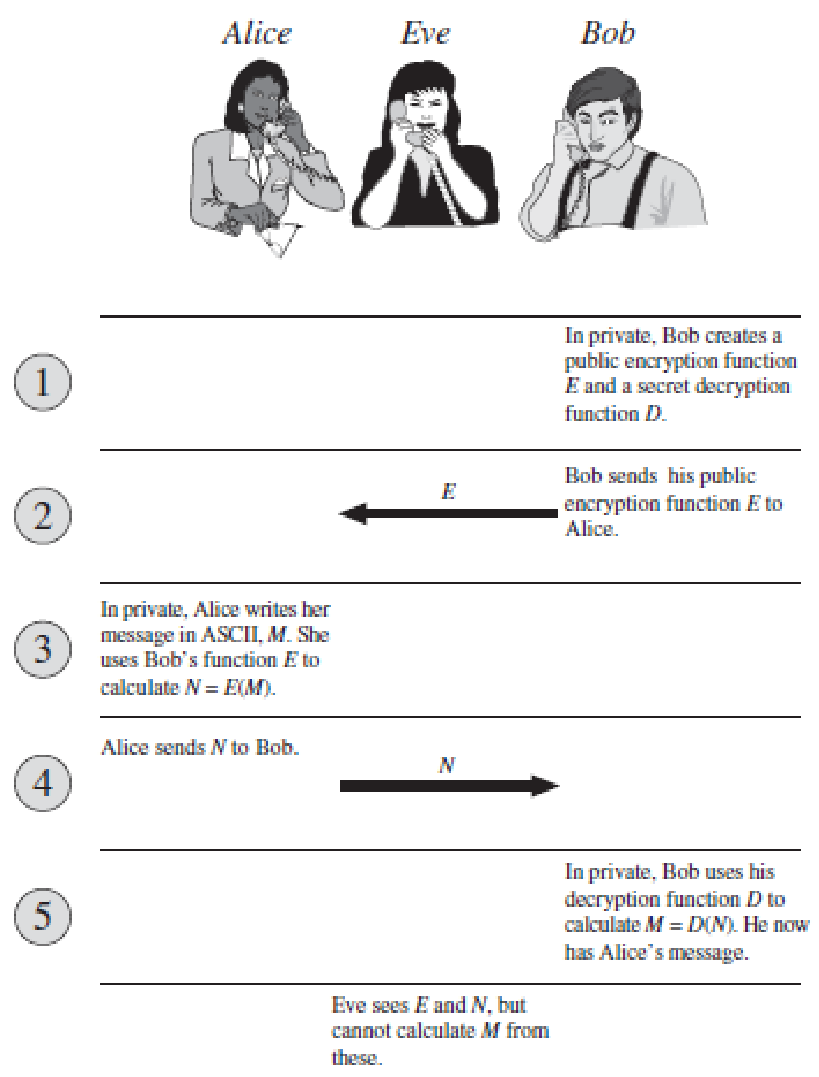
\includegraphics[scale=0.45]{ABE.pdf}
\end{figure}
\end{frame}


\section{Rabin's method}

\begin{frame}{The encryption function}
Let $n$ be a large integer. Set the encryption function to be
\bl[]{\[
E(M)=M^2\textrm{ mod }n
\]}
What should $n$ be?
\itemb
\item If Alice wants to send a message with $c$ characters, then $M$ will have $3c$ digits (up to the initial zeroes) and $M^2$ will have $6c$ digits.
\item If the digits of $n$ is more than $6c$ then $M^2\textrm{ mod }n=M^2$ and Eve can get to the message by computing the ordinary square root.
\item You don't want to loose information so the number of digits of $n$ should be at least $3c$. \vspace{0.2cm}
\iteme
\bl[]{\[
\#\textrm{digits}(M)<\#\textrm{digits}(n)<2\cdot\#\textrm{digits}(M)
\]}
\end{frame}

\begin{frame}{The encryption function}
In our example,
\[
M=73032108105107101032121111117
\]
which has $29$ digits. So if Bob expects such a large message, he can look up two big primes
\[
p=977555333311111,\qquad q=988666444411111 
\]
and multiply them to get
\[
n=966476155599814608692148154321
\]
which will do. This is what Bob sends Alice who then encrypts
\[
N=E(M)=M^2\textrm{ mod }n=412976518048000543454453602839
\]
which she sends back to Bob.
\end{frame}

\begin{frame}{The encryption function}
In our example,
\[
M=73032108105107101032121111117
\]
\[
p=977555333311111,\qquad q=988666444411111 
\]
\[
n=966476155599814608692148154321
\]
\[
N=E(M)=M^2\textrm{ mod }n=412976518048000543454453602839
\]
\itemb
\item Eve now has both $n$ and $N$ but she doesn't have $p$ and $q$. Therefore she cannot invert $E$ to find $D$ and can't extract $M$.
\item Bob knows $p$ and $q$ and $N$ and as we will see, he can invert easily.
\iteme
\end{frame}

\begin{frame}{Square roots in $\mathbb{Z}_n$}
\bl[]{\[
E(M)=M^2\textrm{ mod }n
\]}
If Bob gets $N\in\mathbb{Z}_n$, then to find $M=D(N)$, he needs to take a square root in $\mathbb{Z}_n$.

\begin{center}\color{red} In other words, we need to solve $x\otimes x=N$.\end{center}
For example, by simple brute force
\itemb
\item In $\mathbb{Z}_{59}$, we have $\sqrt{17}=28,31$.
\item In $\mathbb{Z}_{59}$, we have no $\sqrt{18}$.
\item In $\mathbb{Z}_{1121}$, we have $\sqrt{17}=146,500,621,975$.
\item Of course, for huge $n$, this is ridiculous.
\iteme
\end{frame}

\begin{frame}{Quadratic residues}
\bl[]{\[
E(M)=M^2\textrm{ mod }n
\]}
The encrypted message will be  a 'perfect square' in $\mathbb{Z}_n$.
\bl[Definition]{ Let $n$ be a positive integer and let $a\in\mathbb{Z}_n$. If there is an element $b\in\mathbb{Z}_n$ such that $a=b\otimes b$, we call $a$ a \textbf{quadratic residue modulo $n$}. Otherwise we call $a$ a quadratic nonresidue.}
Motivation behind the name:
\[
b\otimes b=b^2\textrm{ mod }n
\]
So $N$ is a quadratic residue modulo $n$.
\end{frame}

%\begin{frame}{Using congruence for computations in $\mathbb{Z}_n$}
%Note that in $\mathbb{Z}_n$,
%\[
%a\otimes b= c\qquad\leftrightarrow \qquad ab \textrm{ mod }n=c.
%\]
%Recall that 
%\[
%a\equiv b\textrm{ (mod $n$)}\qquad \leftrightarrow\qquad a\textrm{ mod }n=b\textrm{ mod } n.
%\]
%Therefore we can perform a computation in $\mathbb{Z}_n$ by working with congruences (\textrm{mod} $n$) in $\mathbb{Z}$ and taking a \textrm{mod} in the end. For example in $\mathbb{Z}_{13}$
%\[
%(7\otimes 6)\oplus 2\equiv 7\cdot 6+2=44\textrm{ (mod 13)}
%\]
%and 
%\[
%(7\otimes 6)\oplus 2=44\textrm{ mod }13=5.
%\]
%\end{frame}

\begin{frame}{Square roots when $n$ is a prime}
Things are relatively simple when $n$ is a prime.
\bl[Proposition]{Let $p$ be a prime and let $a\in\mathbb{Z}_p$. Then $a$ has at most two square roots in $\mathbb{Z}_p$.}
FTSC suppose that $a$ has three (or more) square roots in $\mathbb{Z}_p$. 

~~~~Note that if $x$ is a square root of $a$,
\[
(-x)\otimes (-x)=(-x)^2\textrm{ mod }p=x^2\textrm{ mod }p=x\otimes x = a.
\]
and therefore $-x=0\ominus x$ (in $\mathbb{Z}_p$) is also a square root.

~~~~ Since $a$ has three or more roots, we can choose two of them $x,y\in\mathbb{Z}_p$, such that $x\neq \pm y$. Then
\[
(x-y)(x+y)\textrm{ mod $p$}=x^2-y^2\textrm{ mod $p$}= x^2\ominus y^2=a-a=0
\]
[...]
\end{frame}

\begin{frame}
\bl[Proposition]{Let $p$ be a prime and let $a\in\mathbb{Z}_p$. Then $a$ has at most two square roots in $\mathbb{Z}_p$.}
[...]

~~~~ Since $a$ has three or more roots, we can choose two of them $x,y\in\mathbb{Z}_p$, such that $x\neq \pm y$. Then
\[
(x-y)(x+y)\textrm{ mod $p$}=x^2-y^2\textrm{ mod $p$}= x^2\ominus y^2=a-a=0
\]
But this means that $p|(x-y)(x+y)$, which implies (as $p$ is prime) that
\[
p|(x-y)\qquad\textrm{or}\qquad p|(x+y)
\]
However, since $x\neq \pm y$ and $0\leq x,y<p$, this is not possible. $\Rightarrow\Leftarrow$.\qed
\end{frame}

\begin{frame}{An auxiliary result}
\bl[Fermat's little theorem]{
Let $p$ be a prime and let $a$ be an integer. Then
\[
a^p\equiv a\textrm{ (mod $p$)}
\]}
For example, $5^{23}\equiv 5\textrm{ (mod 23)}$.
\vspace{0.5cm}

This has a generalization:

\bl[Euler's theorem]{Let $n$ be a positive integer and let $a$ be an integer relatively prime to $n$. Then
\[
a^{\varphi(n)}\equiv 1\textrm{ (mod $n$)}
\]}
For proofs, see the textbook.
\end{frame}

\begin{frame}{Identification of quadratic residues in $\mathbb{Z}_p$ for special $p$.}
\bl[Proposition]{Let $p$ be a prime of the form $p=4k+3$ for some $k\in\mathbb{N}$. Let $a\in\mathbb{Z}_p$ be a quadratic residue. Then the square roots of $a$ in $\mathbb{Z}_p$ are
\[
\left[\pm a^{\frac{p+1}{4}}\right]\textrm{ mod }p.
\]}
By the restriction on $p$, $\frac{p+1}{4}$ is an integer and everything makes sense. Since $a$ is a quadratic residue, there is an $x\in\mathbb{Z}_p$ such that $x^2\equiv a$ (\textrm{mod} $p$). Then
\[
\left[\pm a^{\frac{p+1}{4}}\right]^2\equiv \left[x^{\frac{p+1}{2}}\right]^2=x^{p+1}=x^p x\equiv x^2\equiv a\textrm{ (mod $p$)}.
\]
where Fermat's little theorem was used. By the previous Proposition, there are no more roots.\qed
\end{frame}

\begin{frame}{$n=pq$ where $p$ and $q$ are primes of the form $4k+3$.}
We still want to solve $x\otimes x=N$ in $\mathbb{Z}_n$. This is the same as
\[
x^2\textrm{ mod $n$}=N
\]
which means that for some $k\in\mathbb{Z}$,
\[
x^2=kn+N=k(pq)+N
\]
But this means both
\[
x^2=(kp)q+N,\qquad x^2=(kq)p+N
\]
or
\[
x^2\textrm{ mod $p$}=N\qquad x^2\textrm{ mod $q$}=N.
\]
But if $x_1$ is a square root of $N$ in $\mathbb{Z}_{p}$ and $x_2$ is a square root of $N$ in $\mathbb{Z}_{q}$ (which we now know how to compute for our special primes), then an $x$ satisfying both
\[
x=x_1+k_1q\qquad x=x_2+k_2p
\]
for some $k_1,k_2\in\mathbb{Z}$ does the job.
\end{frame}

\begin{frame}{In our example}
For Bob's public key
\[
n=966476155599814608692148154321
\]
he has that
\[
p=977555333311111,\qquad q=988666444411111 
\]
are both of the form $4k+3$ and therefore
\itemb
\item $\sqrt{N}$ in $\mathbb{Z}_{p}$ is
\[
\pm N^{\frac{p+1}{4}}\textrm{ mod }p=\pm N^{244388833327778}\textrm{ mod }p=\pm 869000357225117
\]
\item $\sqrt{N}$ in $\mathbb{Z}_{q}$ is
\[
\pm N^{\frac{q+1}{4}}\textrm{ mod }q=\pm N^{988666444411111}\textrm{ mod }q=\pm 154623490704086
\]
\iteme
In other words
\[
x_1= 869000357225117, 108554976085994
\]
\[
x_2=154623490704086, 834042953707025
\]
\end{frame}

\begin{frame}{Chinese remainder theorem}\vspace{-0.5cm}
\[
x_1= 869000357225117, 108554976085994
\]
\[
x_2=154623490704086, 834042953707025
\]
This gives four equation of the form
\[
x=x_1+k_1p\qquad x=x_2+k_2q
\]\vspace{-0.6cm}\\
or in other words\vspace{-0.1cm}
\[
x\equiv x_1\textrm{ (mod $p$)},\qquad x\equiv x_2 \textrm{ (mod $q$)}
\]\vspace{-0.5cm}
\bl[Chinese remainder theorem]{
The pair of congruences
\[
x\equiv x_1\textrm{ (mod $p$)},\qquad x\equiv x_2 \textrm{ (mod $q$)}
\]
has a unique solution $x_0$ with $0\leq x_0<pq$. Furthermore, every mutual solution to these congruences differs from $x_0$ by a multiple of $mn$.
}
\end{frame}

\begin{frame}{In our example}
We earlier got
\[
x_1= 869000357225117, 108554976085994
\]
\[
x_2=154623490704086, 834042953707025
\]
If $p^{-1}$ is the reciprocal of $p$ in $\mathbb{Z}_q$,
\[
M=x_0=x_1+\left[((x_2-x_1)\textrm{ mod } q)\otimes p^{-1}\right]p\textrm{ mod }n
\]
Two independent possibilites for $x_1$ and $x_2$ gives us four $x_0$-s.

The Euclidean algorithm yields
\[
-174529541694500p+172568094394491q=1
\]
and thus in $\mathbb{Z}_q$,
\[
p^{-1}=-174529541694500\textrm{ mod }q=814136902716611
\]
\end{frame}

\begin{frame}{In our example}
We earlier got
\[
x_1= 869000357225117, 108554976085994
\]
\[
x_2=154623490704086, 834042953707025
\]
For each pair $x_1,x_2$,
\[
M=x_1+\left[((x_2-x_1)\textrm{ mod } q)\otimes p^{-1}\right]p\textrm{ mod }n
\]
\[
p^{-1}=814136902716611
\]
This gives the following four $M$ values:
\[
M_1=73032108105107101032121111117
\]
\[
M_2=811685135902651145620250169817
\]
\[
M_3=893444047494707507660027043204
\]
\[
M_4=154791019697163463071897984504
\]
\end{frame}

\begin{frame}{In our example}
This gives the following four $M$ values:
\[
M_1=73032108105107101032121111117
\]
\[
M_2=811685135902651145620250169817
\]
\[
M_3=893444047494707507660027043204
\]
\[
M_4=154791019697163463071897984504
\]
To see if any of this is the actual message, do inverse ASCII:
\[
M_1\to \textrm{ I like you}\qquad
M_2\to Junk\qquad
M_3\to Junk\qquad
M_4\to Junk
\]
So the message is clearly discernable for Bob.
\end{frame}

\begin{frame}{Summary}
After Bob gets $N$,
\itemb
\item Compute $\sqrt{N}$ in $\mathbb{Z}_p$ and $\mathbb{Z}_q$.
\item This gives four pairs for $(x_1,x_2)$.
\item For each pair solve the Chinese remainder problem and get an $M$. 
\item Out of the four $M$-s, three will be gibberish, the remaining one is the original $M$.
\iteme
\end{frame}


\section{The RSA method}
\begin{frame}{Euler's totient}
\bl[Definition]{For every positive integer $n$, let $\varphi(n)$ denote the number of integers from $1$ to $n$ inclusive that are relatively prime to $n$.}
For example,
\itemb
\item For $n=14$, $\{1,3,5,9,11,13\}$ are the relative primes to $n$ and therefore $\varphi(14)=6$.
\item For $n=15$, $\{1,2,4,7,8,11,13,14\}$ are the relative primes to $n$ and therefore $\varphi(15)=8$.
\iteme
\bl[Theorem]{If the prime factorization of $n$ is $p_1^{a_1}p_2^{a_2}\dots p_t^{a_t}$, then
\[
\varphi(n)=n\left(1-\frac{1}{p_1}\right)\left(1-\frac{1}{p_2}\right)\dots \bigg(1-\frac{1}{p_t}\bigg)
\]
}
\end{frame}


\begin{frame}{Euler's totient}
\bl[Theorem]{If the prime factorization of $n$ is $p_1^{a_1}p_2^{a_2}\dots p_t^{a_t}$, then
\[
\varphi(n)=n\left(1-\frac{1}{p_1}\right)\left(1-\frac{1}{p_2}\right)\dots \bigg(1-\frac{1}{p_t}\bigg)
\]
}
\begin{figure}
\centering
\includegraphics[scale=0.6]{Euler.jpg}
\end{figure}
%\bl[Fact]{$|\mathbb{Z}_n^*|=\varphi(n)$.}
\end{frame}

\begin{frame}{An auxiliary result}
\bl[Fermat's little theorem]{
Let $p$ be a prime and let $a$ be an integer. Then
\[
a^p\equiv a\textrm{ (mod $p$)}
\]}
For example, $5^{23}\equiv 5\textrm{ (mod 23)}$.
\vspace{0.5cm}

This has a generalization:

\bl[Euler's theorem]{Let $n$ be a positive integer and let $a$ be an integer relatively prime to $n$. Then
\[
a^{\varphi(n)}\equiv 1\textrm{ (mod $n$)}
\]}
For proofs, see the textbook.
\end{frame}

\begin{frame}{The encryption function}
\bl[]{
\[
E(M)=M^e\textrm{ mod }n,\qquad D(N)=N^d\textrm{ mod }n
\]}
for appropriately chosen $e$ and $d$ and $n=pq$ as before.
\[
D(E(M))=D(M^e\textrm{ mod }n)=M^{ed}\textrm{ mod }n
\]
By Euler's theorem, we know that 
\[
M^{\varphi(n)}=1\qquad\textrm{in }\mathbb{Z}_n
\]
and therefore
\[
M^{k\varphi(n)+1}=(M^{\varphi(n)})^kM=1^kM=M\qquad\textrm{in }\mathbb{Z}_n
\]
and so we want $ed=k\varphi(n)+1$.
\end{frame}

\begin{frame}{The encryption function}
\bl[]{
\[
E(M)=M^e\textrm{ mod }n,\qquad D(N)=N^d\textrm{ mod }n
\]}
We want $ed=k\varphi(n)+1$. 
\itemb
\item Since Bob knows $p$ and $q$, he can compute $\varphi(n)$ easily. 
\item Bob selects his favorite $e\in\mathbb{Z}_{\varphi(n)}$. 
\item Then he computes $d=e^{-1}\in\mathbb{Z}_{\varphi(n)}$.
\item He tells Alice $n$ and $e$ publicly (so that Eve can hear), but keeps $p,q$ and $d$ a secret.
\item Alice computes $N=E(M)$ using Bob's key and sends $N$ to Bob.
\item Eve knows $n$, $e$, but he cannot find $D(N)$ as he can't find $\varphi(n)$.
\item Bob decodes $M=D(N)$ and they live happily ever after.
\iteme
\end{frame}
\end{document}